\section{RTL Implementation Strategy}

\subsection{IEEE 754 Single-Precision Floating-Point Adder/Subtractor Design}

\begin{figure}[H]
	\centering
	\includegraphics[height=\linewidth, scale=0.5]{./../Version2/02_rtl/FPU_ADD_SUB/00_spec/Flowchart_for_FPU_ADD_SUB.png}
	\caption{Algorithmic flowchart of the IEEE 754 Floating-Point Adder/Subtractor.}
	\label{fig:fpu_add_sub_flowchart}
\end{figure}

\begin{figure}[H]
	\centering
	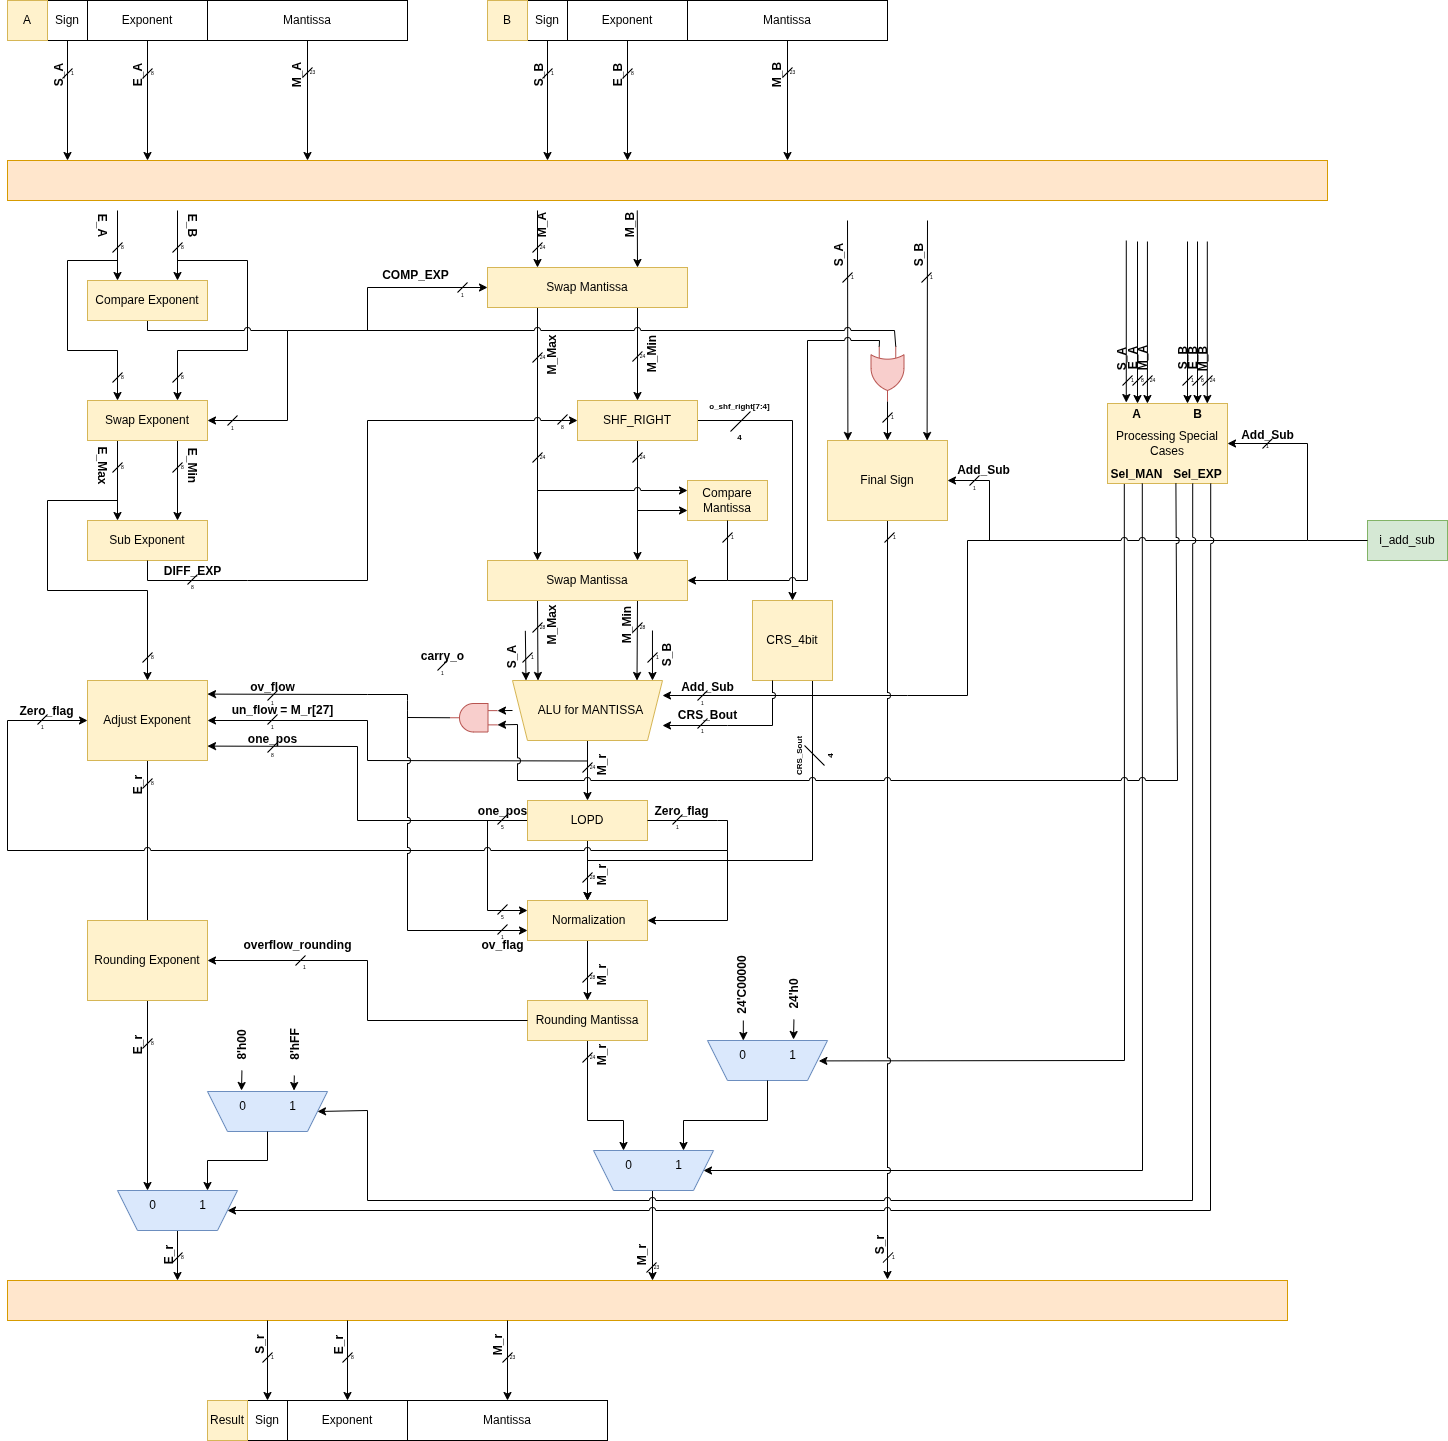
\includegraphics[width=.9\linewidth]{./../Version2/02_rtl/FPU_ADD_SUB/00_spec/BlockDiagram_Overview.png}
	\caption{Top-level hardware architecture of the 32-bit Floating-Point Adder/Subtractor.}
	\label{fig:fpu_add_sub_block_diagram}
\end{figure}

\subsection{IEEE 754 Single-Precision Floating-Point Multiplier Design}

\begin{figure}[H]
	\centering
	\includegraphics[height=\linewidth, scale=0.5]{./../Version2/02_rtl/FPU_MUL/00_spec/Flowchart_for_FPU_MUL.png}
	\caption{Algorithmic flowchart of the IEEE 754 Floating-Point Multiplier.}
	\label{fig:fpu_mul_flowchart}
\end{figure}

\begin{figure}[H]
	\centering
	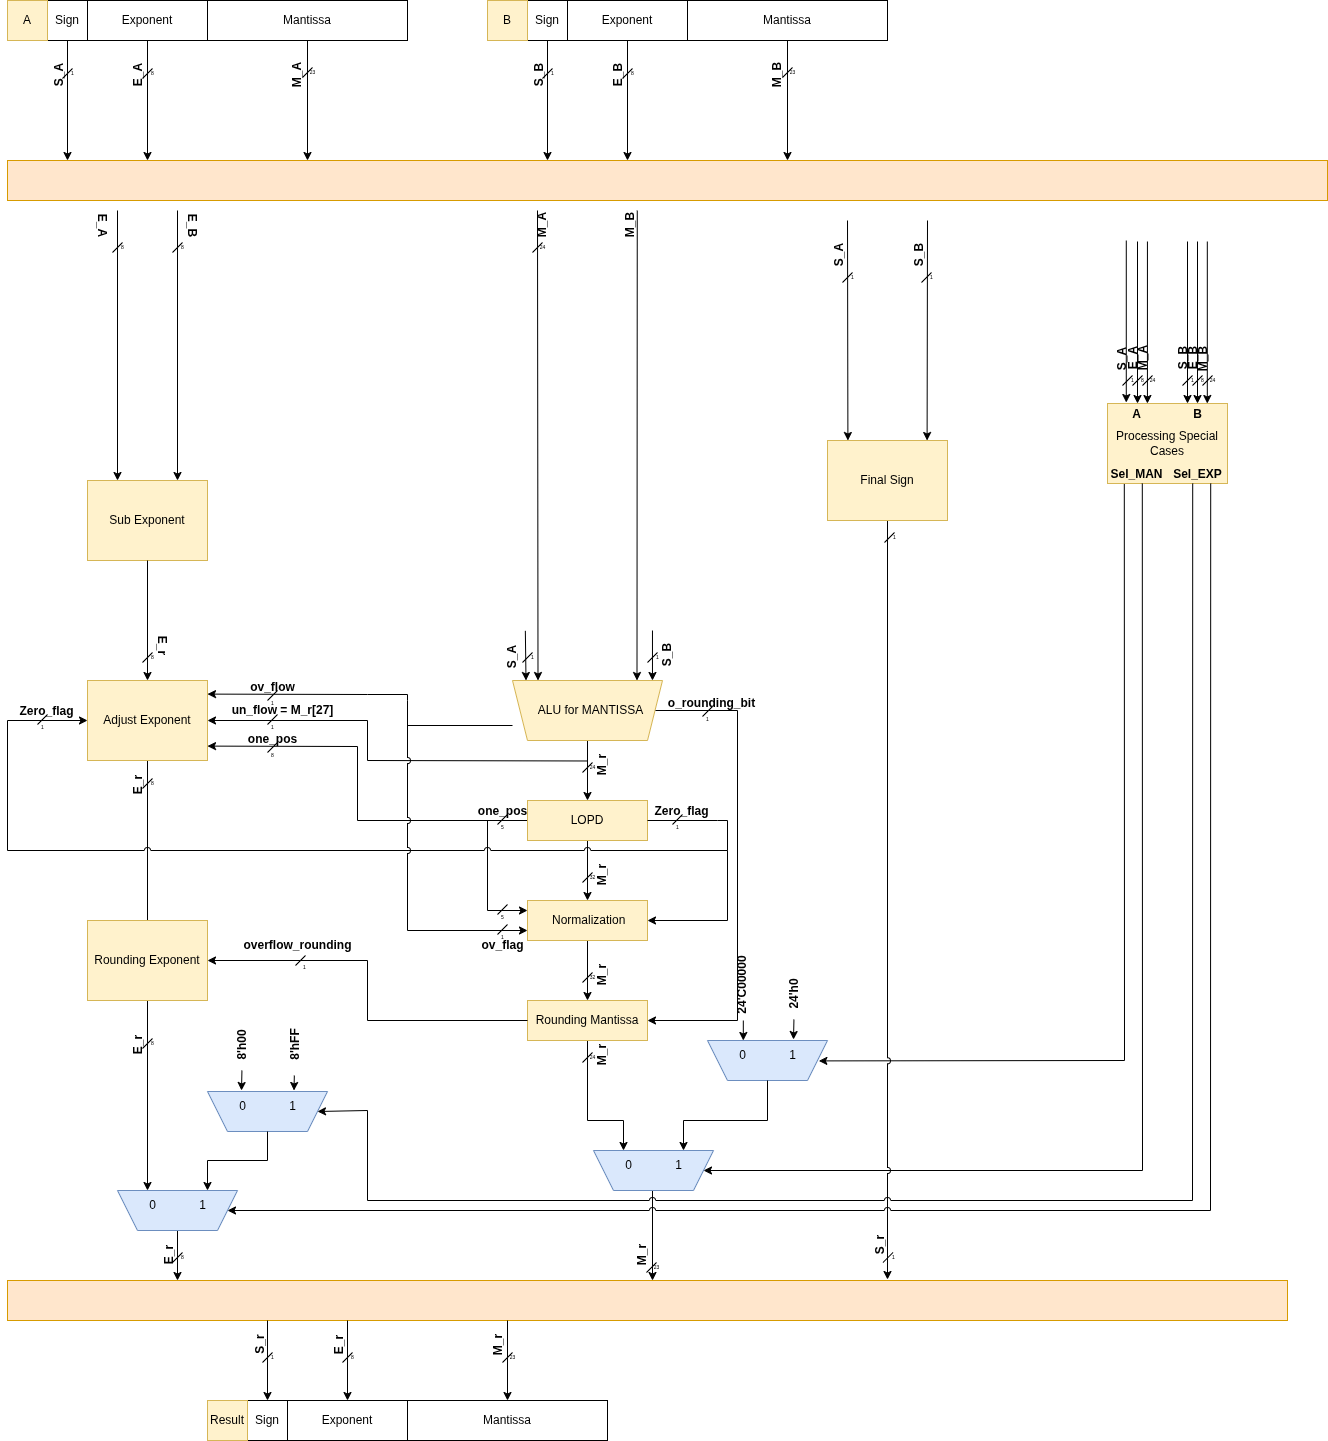
\includegraphics[width=.9\linewidth]{./../Version2/02_rtl/FPU_MUL/00_spec/BlockDiagram_Overview.png}
	\caption{Top-level hardware architecture of the 32-bit Floating-Point Multiplier.}
	\label{fig:fpu_mul_block_diagram}
\end{figure}

\subsection{8-Point FFT Processor Top-Level Architecture}

\subsubsection{Thiết kế bộ FFT nguyên bản}

Đầu tiên, ta thiết kế một bộ Butterfly Processor Unit thực hiện phép nhân số phức như sau:

\[ (a + jb)*(c + jd) = ac + jad + jbc - bd = (ac - bd) + j(ad + bc) \]

\begin{figure}[H]
	\centering
	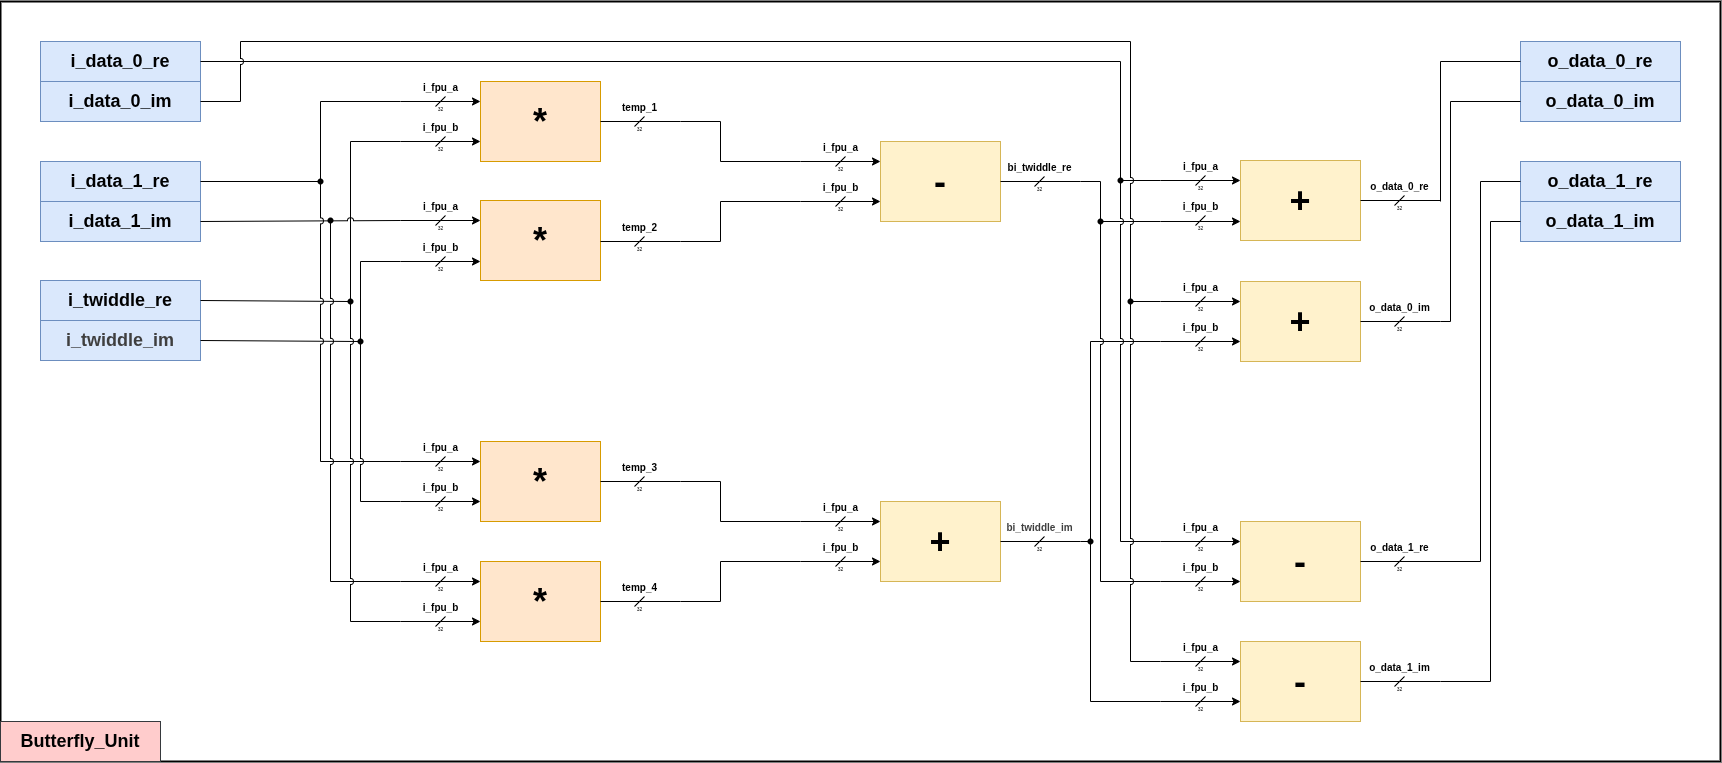
\includegraphics[width=.8\linewidth]{./../Version2/02_rtl/ButterFly/00_spec/Butterfly_unit.png}
	\caption{Structure of Radix-2 Butterfly Processing Unit (BPU).}
\end{figure}

Sử dụng bộ trên để thực hiện theo bộ tính FFT theo sơ đồ như sau:

\begin{figure}[H]
	\centering
	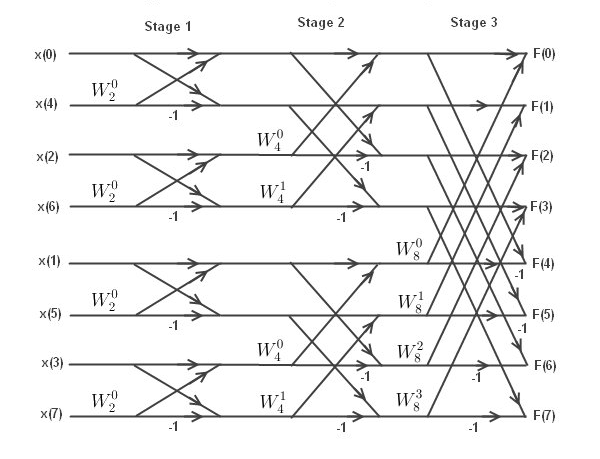
\includegraphics[width=.7\linewidth]{./my-chapters/my-images/DesignRTL_FFT/FFT_original.png}
\end{figure}

Từ đó, ta có thiết kế RTL như sau:

\begin{figure}[H]
	\centering
	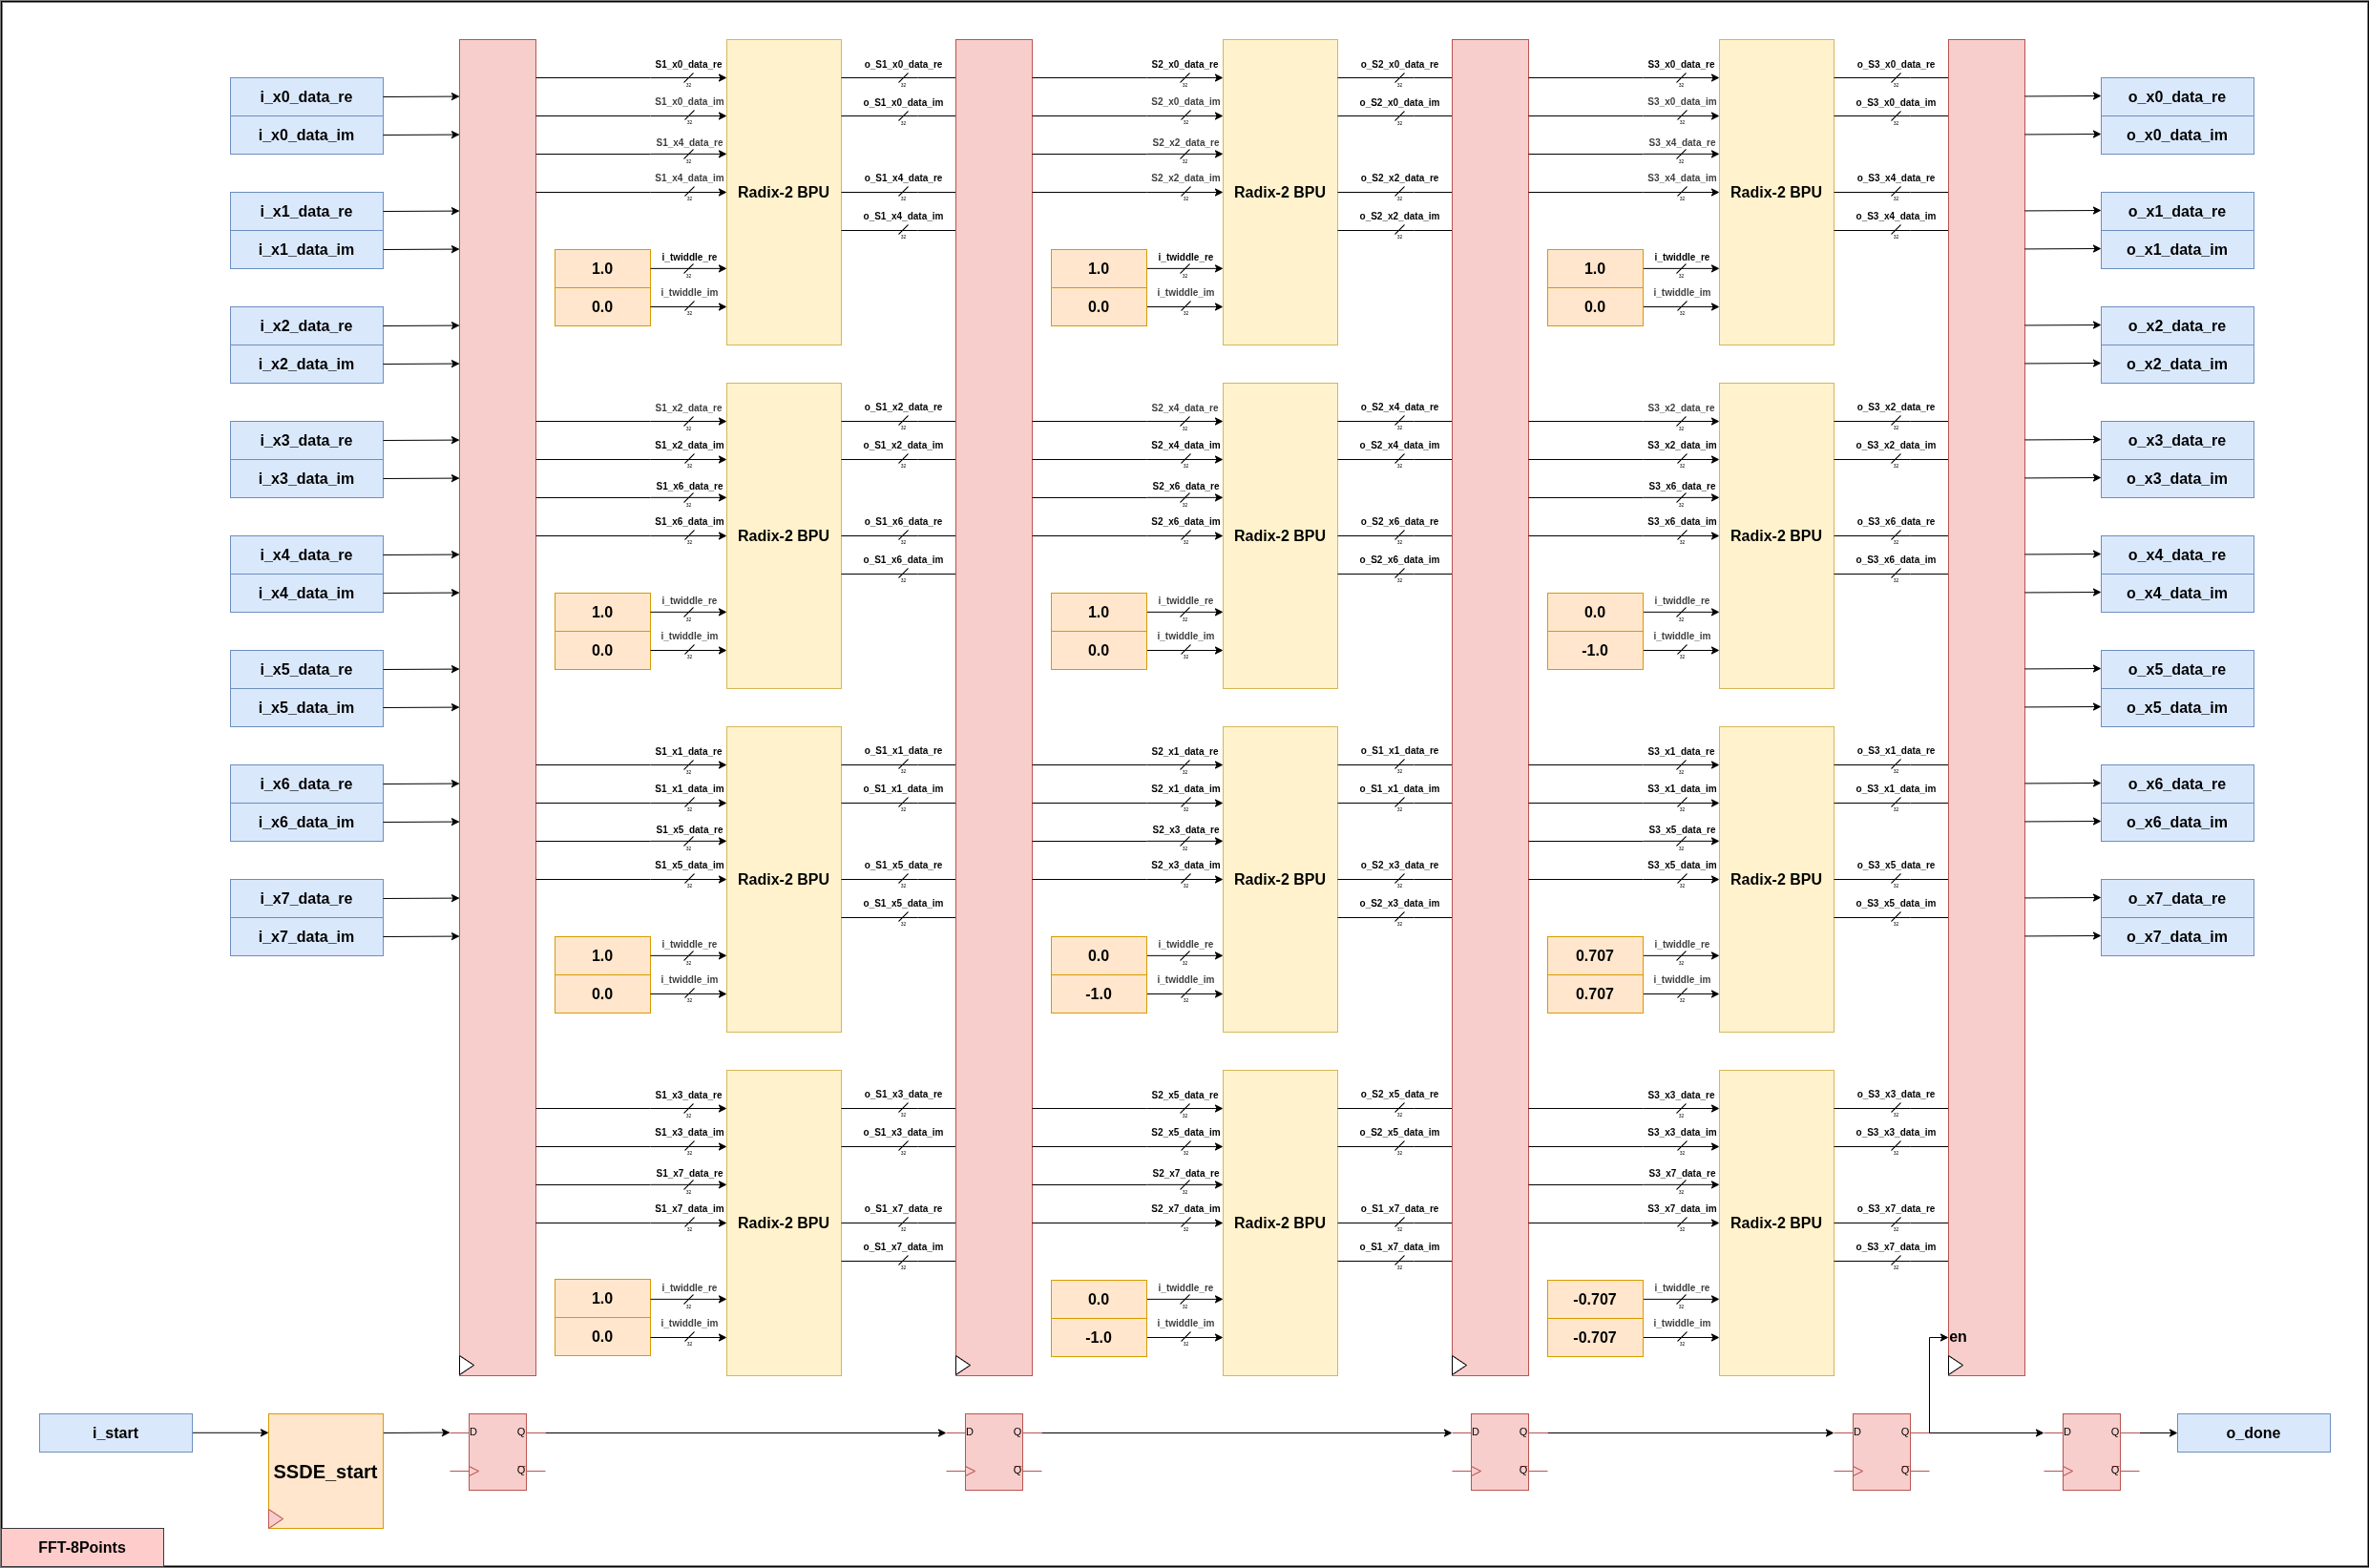
\includegraphics[width=.8\linewidth]{./../Version2/02_rtl/FFT_unit/00_spec/FFT_8Point.png}
	\caption{Structure of 8-Point FFT Processor Original.}
	\label{fig: FFT_8point}
\end{figure}

Tuy nhiên, với thiết kế \ref{fig: FFT_8point} thì sử dụng đến 12 bộ Butterfly Processor Unit (BPU) trong thiết kế tổng, như vậy cần sử dụng đến:

\begin{itemize}
	\item Bộ cộng/trừ: 72 bộ.
	\item Bộ nhân: 48 bộ.
\end{itemize}

Như vậy, với thiết kế nguyên bản sử dụng rất nhiều tài nguyên.

\subsubsection{Thiết kế bộ FFT sau khi tối ưu hóa}

Ta thấy khi sử dụng kiến trúc FFT 8-Point như hình \ref{fig: FFT_8point}, ta nhận thấy có các vị trí trong vòng tròn pha (Twiddle) có các giá trị như:

\begin{itemize}[label=-]
	\item $W_8^0 = 1$
	\item $W_8^1 = \cos(\frac{\pi}{4}) - j\sin(\frac{\pi}{4}) = \frac{\sqrt{2}}{2} - j\frac{\sqrt{2}}{2} \approx 0.7071 - j0.7071$
	\item $W_8^2 = -j$
	\item $W_8^3 = \cos(\frac{3\pi}{4}) - j\sin(\frac{3\pi}{4}) = -\frac{\sqrt{2}}{2} - j\frac{\sqrt{2}}{2} \approx -0.7071 - j0.7071$
\end{itemize}

\begin{enumerate}[label=\arabic*.]
	\item Ở tầng 1:
		\begin{figure}[H]
			\centering
			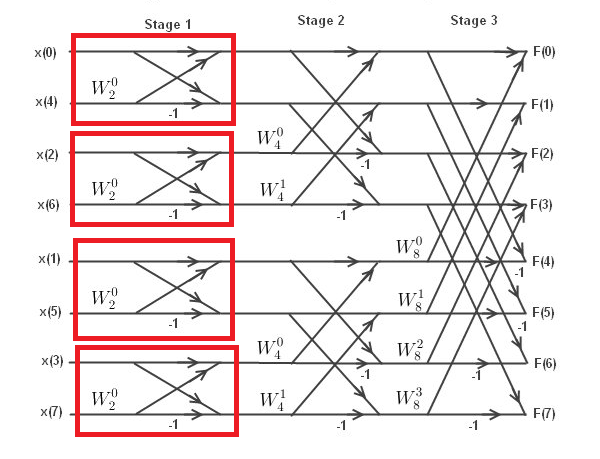
\includegraphics[width=alt=.6\linewidth]{./my-chapters/my-images/DesignRTL_FFT/FFT_cus_BF2.png}
		\end{figure}
		
		Các Butterfly chỉ nhân với giá trị $W^{0}_{2} = 1$ nghĩa là không cần sử dụng bộ nhân trong thiết kế. Vì thế ta có thể thiết kế bộ BPU ở tầng 1 như sau:
		\begin{figure}[H]
			\centering
			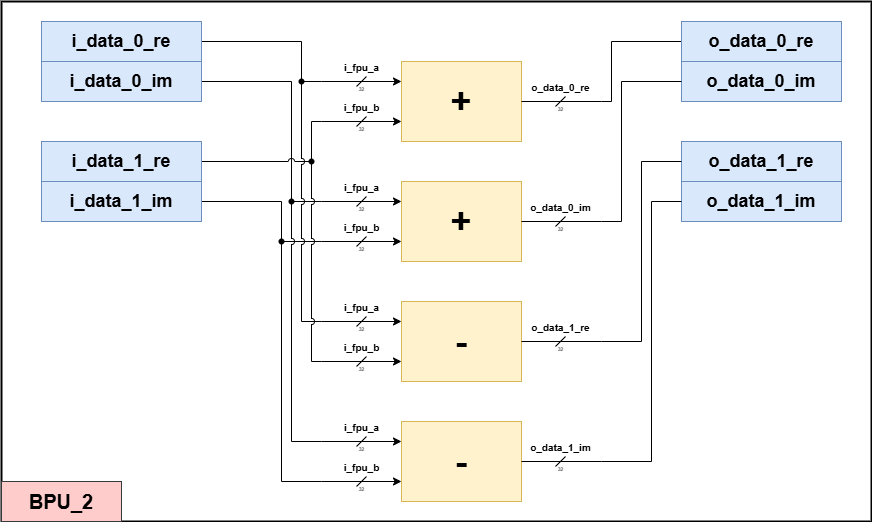
\includegraphics[width=.7\linewidth]{./../Version2/02_rtl/ButterFly/00_spec/BFP_2.png}
			\caption{Bộ BFP ở tầng 1 của bộ FFT.}
		\end{figure}
		
	\item Ở tầng 2:
	\begin{figure}[H]
		\centering
		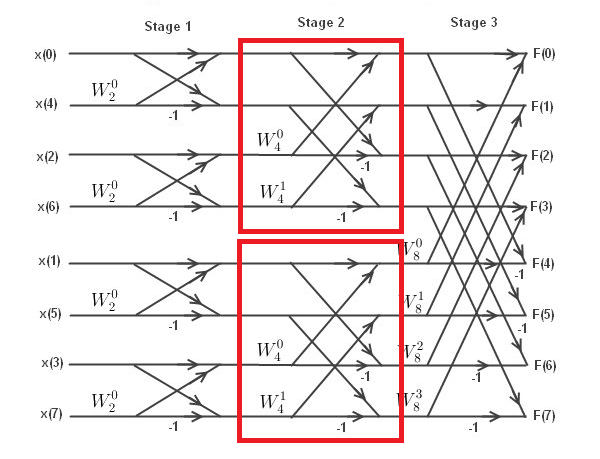
\includegraphics[width=alt=.6\linewidth]{./my-chapters/my-images/DesignRTL_FFT/FFT_cus_BF4.png}
	\end{figure}
	
	Các Butterfly cần xử lý hai giá trị của Twddile là $W^{0}_{4} = 1$ và $W^{1}_{4} = -j$. Với giá trị $W^{0}_{4} = 1$ thì ta thực hiện tương tự như bộ BPU ở tầng 1, còn giá trị $W^{1}_{4} = -j$ thì ta nhận thấy khi:
	\[ (a + jb) * (-j) = b - ja\]
	Có nghĩa là giá trị tại $X(6)$ sẽ đảo giá trị vị trí phần thực và phần ảo với nhau và thực hiện bù dấu cho phần ảo.
	
	\begin{figure}[H]
		\centering
		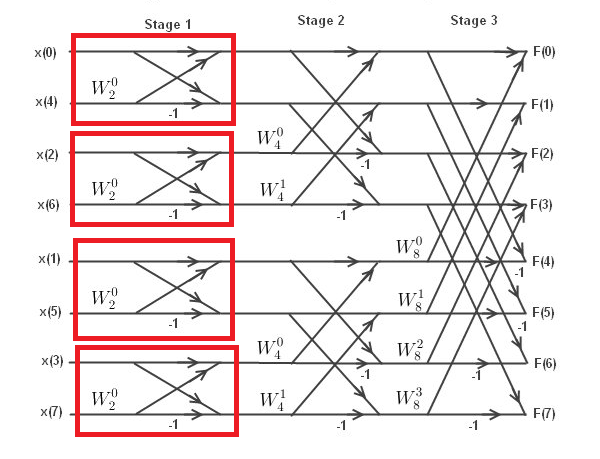
\includegraphics[width=.7\linewidth]{./my-chapters/my-images/DesignRTL_FFT/FFT_cus_BF2.png}
		\caption{Bộ BFP ở tầng 3 của bộ FFT.}
	\end{figure}
	
	\item Ở tầng 3:
	
\end{enumerate}
